\subsection{Активация устройства}
\label{sec:usage:deviceactivation}

После успешного подтверждения телефона, пользователь может попасть на~один из~двух экранов:

\begin{enumerate}
	\item Экран списка диалогов. Пользователь попадает на~этот экран, если текущее устройство является первым устройством, которое регистрируется на~указанный ранее номер.
	\item Экран активации устройства. Если у пользователя уже имеются активные устройства, приложение переходит на~экран активации устройства, показанный на~рисунке \ref{sec:usage:deviceactivation:ui} A.
\end{enumerate}

Если пользователь попал на~экран активации устройства -- значит на~его остальные устройства было отправлено уведомление с~просьбой активировать новое устройство, которое изображено на~рисунке \ref{sec:usage:deviceactivation:ui} Б. Пользователь должен нажать <<Разрешить>> на~любом другом устройстве для~продолжения использования приложения на~новом устройстве.

\begin{figure}[h]
  \centering
    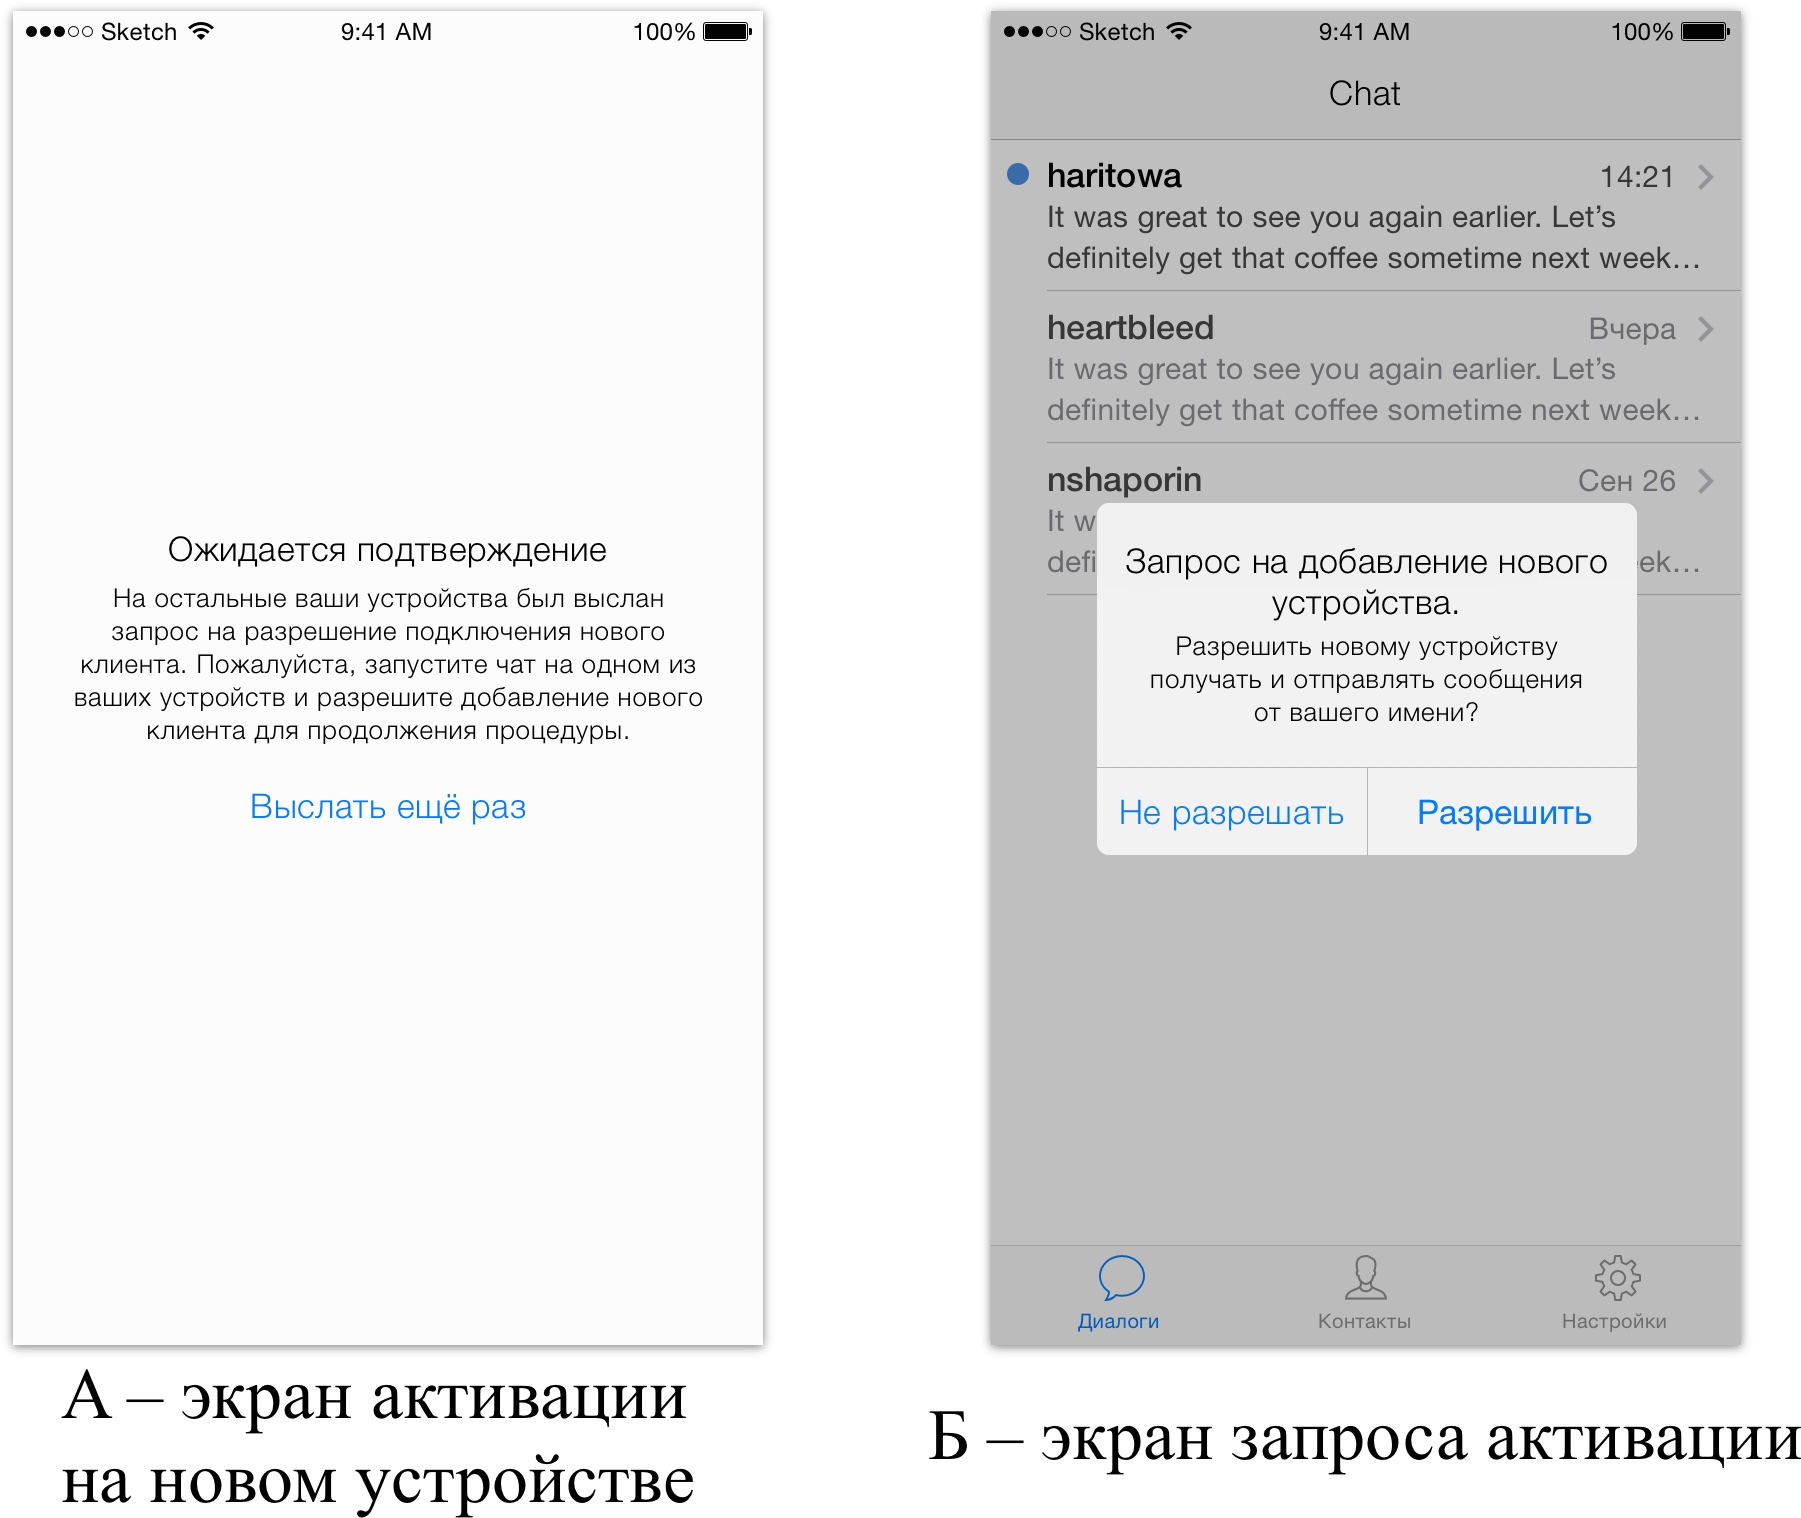
\includegraphics[width=0.75\textwidth]{inc/img/ui/ui_approve.jpg}
  \caption{Экраны активации нового устройтсва}
  \label{sec:usage:deviceactivation:ui}
\end{figure}

При проектировании программного средства, особое внимание уделялось безопасности и~надёжности, продумывалась масса неординарных сценариев. Подход с~активацией устройства показал себя лучшим компромисом, предоставляющим высокий уровень безопасности.